\documentclass[journal]{IEEEtran}

% Packages
\usepackage{cite}
\usepackage{graphicx}
\usepackage{subfigure}
\usepackage{float}
\usepackage{url}
\usepackage{color}


\begin{document}

% paper title
% can use linebreaks \\ within to get better formatting as desired
\title{Autonomous~Robotics~Lab~3 \\ Path~Planning~With~RRT}
%

\author{Rodrigo~Caye~Daudt}





% make the title area
\maketitle



%%%%%%%%%%%%%%%%%%%%%%%%%%%%%%%%%%%%%%%%%%%%%%%%%%%%%%%%%%%%%%%%%%%%%%%%%%%%%%%
\section{Introduction}

\IEEEPARstart{T}{his} report describes the work done for lab 3 of the Autonomous Robotics module. The objective here was to develop a MATLAB function to apply the Rapid exploring random trees (RRT) algorithm for planning a path between a starting position and a goal point using a known map.

Section \ref{rrt} describes in detail the RRT algorithm and gives some information about the developed implementation. Section \ref{results} contains the results and analysis for a few example environments. Section\ref{conclusion} concludes this work by highlighting the main points of this work.

%%%%%%%%%%%%%%%%%%%%%%%%%%%%%%%%%%%%%%%%%%%%%%%%%%%%%%%%%%%%%%%%%%%%%%%%%%%%%%%
\section{RRT Algorithm And Implementation Details}\label{rrt}

RRT is a Monte Carlo method used for finding a path between two points in a given map. It uses random sampling to generate a tree of valid linear path segments that ideally connect the two points. Our implementation here is a simple version or RRT, where only one tree is grown from the starting position to the goal point.

The implemented \textit{rrt}, which can be found in Appendix \ref{aprrt} function has the following input parameters:
\begin{itemize}
	\item \textbf{map} - The grid map of the environment. It assumes that 0 means a clear path and 1 means an object exists at that position.
	\item \textbf{q\_start} - $(x,y)$ coordinates of the starting position.
	\item \textbf{q\_goal} - $(x,y)$ coordinates of the goal point.
	\item \textbf{k} - Maximum number of iterations of the algorithm before it gives up. This is used to avoid getting stuck in an infinite loop when a path is not found.
	\item \textbf{delta\_q} - Parameter that controls the distance of each step.
	\item \textbf{p} - Probability of using \textit{q\_goal} to generate the next tree point candidate.
\end{itemize}

The outputs of the \textit{rrt} function are:
\begin{itemize}
	\item \textbf{vertices} - The list of the coordinates of all the nodes generated by the RRT algorithm.
	\item \textbf{edges} - The connexions between the nodes in the \textit{vertices} list.
	\item \textbf{path}\footnote{In the lab sheet, it is asked for the path to go from \textit{q\_start} to \textit{q\_goal}, but the given example goes in the opposite direction. Since it was ambiguous, the \textit{rrt} function generated a path starting in \textit{q\_start} and ending in \textit{q\_goal}, since that is the more intuitive approach.} - The path between \textit{q\_start} and \textit{q\_goal} found by the RRT algorithm. If no path is found, this is an empty list.
\end{itemize}

The RRT algorithm starts at \textit{q\_start} in its vertices list as the original node of the tree. At each iteration, a random point called \textit{q\_random} in the free space is sampled. The \textit{p} parameter defines how often \textit{q\_random} will be chosen as \textit{q\_goal}. All the points in the vertices list are compared to \textit{q\_random} to find the nearest point \textit{q\_near}. Afer \textit{q\_near} is found, a point \textit{q\_new} is generated at a distance \textit{delta\_q} from \textit{q\_near} in the direction of \textit{q\_random} to serve as a candidate point. 

After the coordinates of \textit{q\_new} are calculated, the visibility between \textit{q\_near} and \textit{q\_new} is checked by checking at least 10 points between them. If any of this points belongs to an obstacle in the map, \textit{q\_near} and \textit{q\_new} are considered to be not visible to each other. Otherwise, if all the checked points between \textit{q\_near} and \textit{q\_new} are valid path points they are considered visible to each other. If this is the case, \textit{q\_new} is added to the vertices list and an edge between \textit{q\_near} and \textit{q\_new} is added to the edges list.

After a new point has been added to the vertices list, we check if the distance between \textit{q\_new} and \textit{q\_goal} is smaller than \textit{delta\_q}, and if so we check if they are visible to each other in the same way that was previously described. If both these conditions are met, \textit{q\_goal} is added to the vertices list, the edge between \textit{q\_new} and \textit{q\_goal} is added to the edges list and the loop that generates the tree is terminated since the goal has been reached.

Once the goal has been reached, the path that leads from \textit{q\_start} to \textit{q\_goal} is generated by propagating back from \textit{q\_goal} using the edges list until \textit{q\_start} is reached, generating a valid path between the two desired points. If the maximum number of iterations has been reached by the tree generating loop, the algorithm is terminated with an empty path, meaning no valid path has been found between the two points.

Since RRT is a stochastic method, its results are not guaranteed, and if a result is found it is also not an optimal result. To improve the results of our \textit{rrt} function, a \textit{smooth} function has been implemented to improve the path generated by the RRT algorithm, which can be found in Appendix \ref{apsmooth}. This function eliminates useless points from the RRT path by checking the farthest visible node to each node in the path, and eliminates all the points in between. This results in a shorter path with less nodes between \textit{q\_start} and \textit{q\_goal}, and helps prevent weird behaviours in the RRT generated paths.



%\begin{figure}
%	\centering
%	\includegraphics[width=0.8\linewidth]{figures/blocks.png}
%	\caption{Illustration }
%	\label{blocks}
%\end{figure}








%%%%%%%%%%%%%%%%%%%%%%%%%%%%%%%%%%%%%%%%%%%%%%%%%%%%%%%%%%%%%%%%%%%%%%%%%%%%%%%
\section{Results and Discussion}\label{results}


\begin{figure*}[p]
	\centering
	
	\subfigure[Map result with delta\_q=50]{\label{map50}
		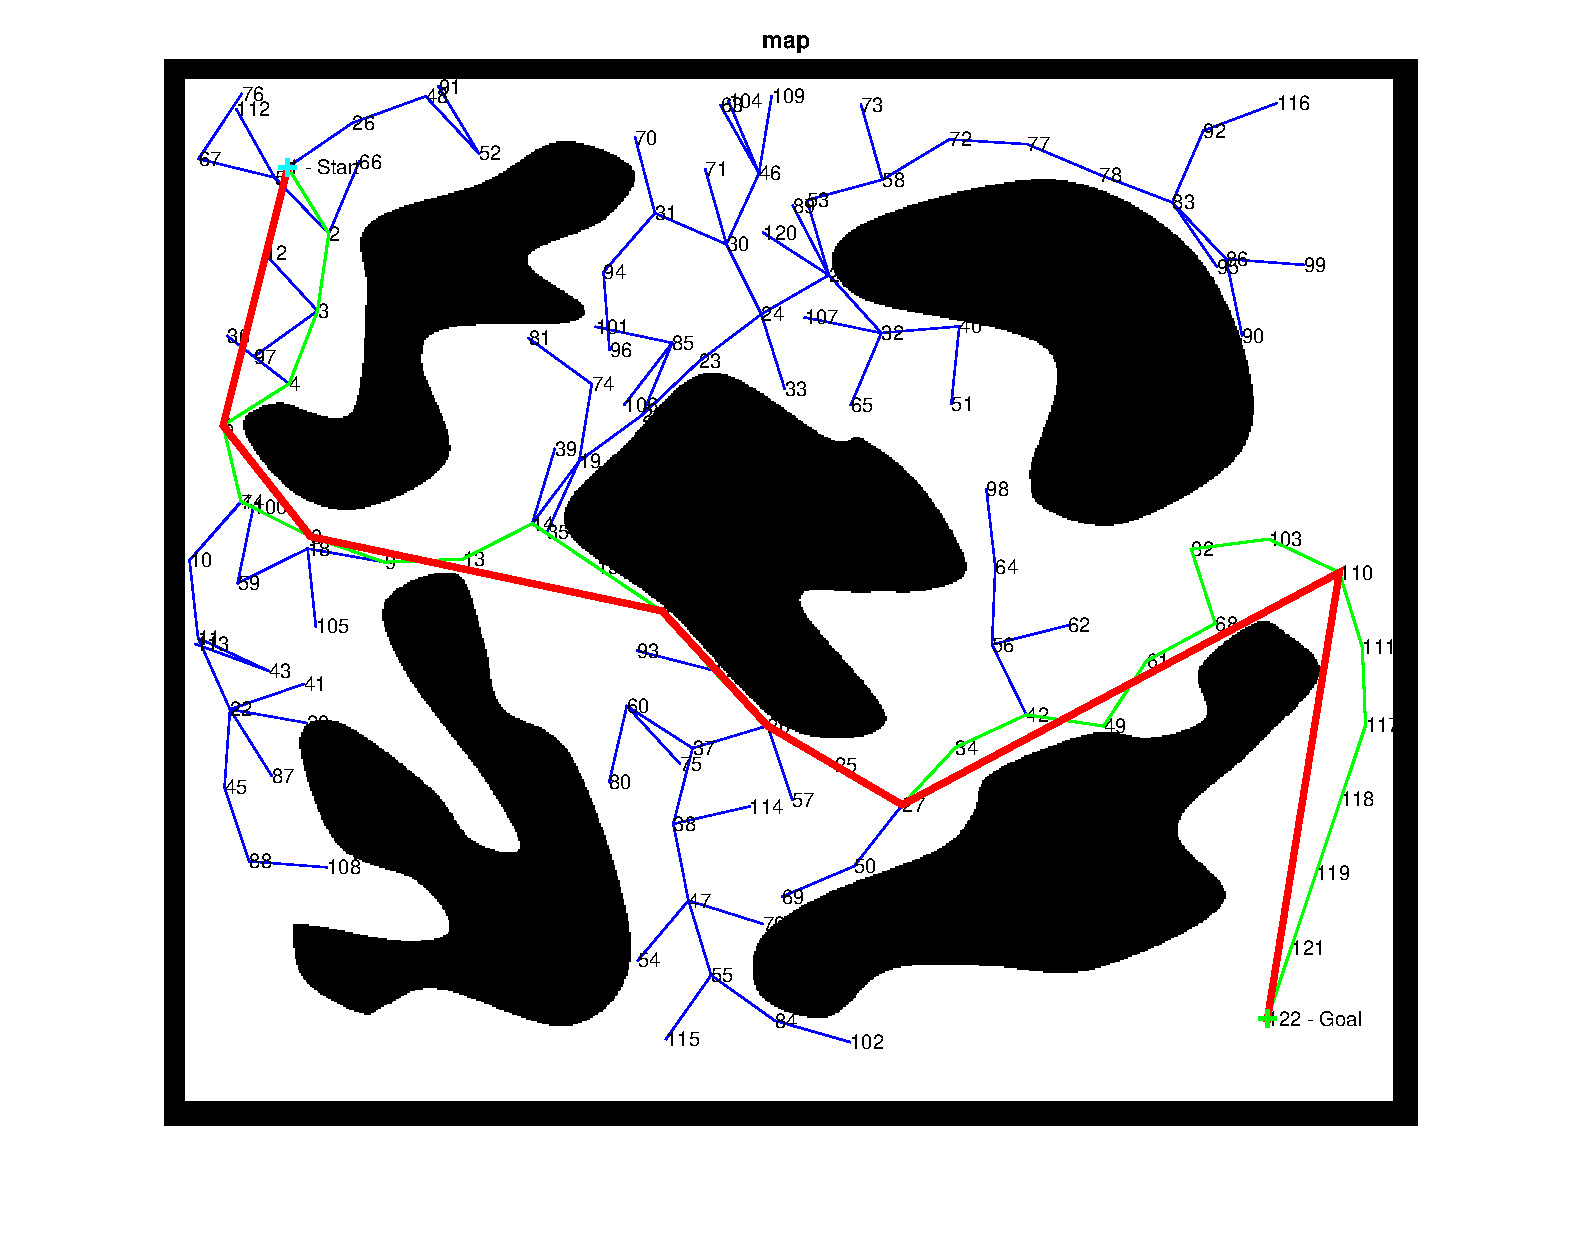
\includegraphics[width=0.45\linewidth]{figures/map_50_03.eps}}~
	\subfigure[Maze result with delta\_q=50]{\label{maze50}	
		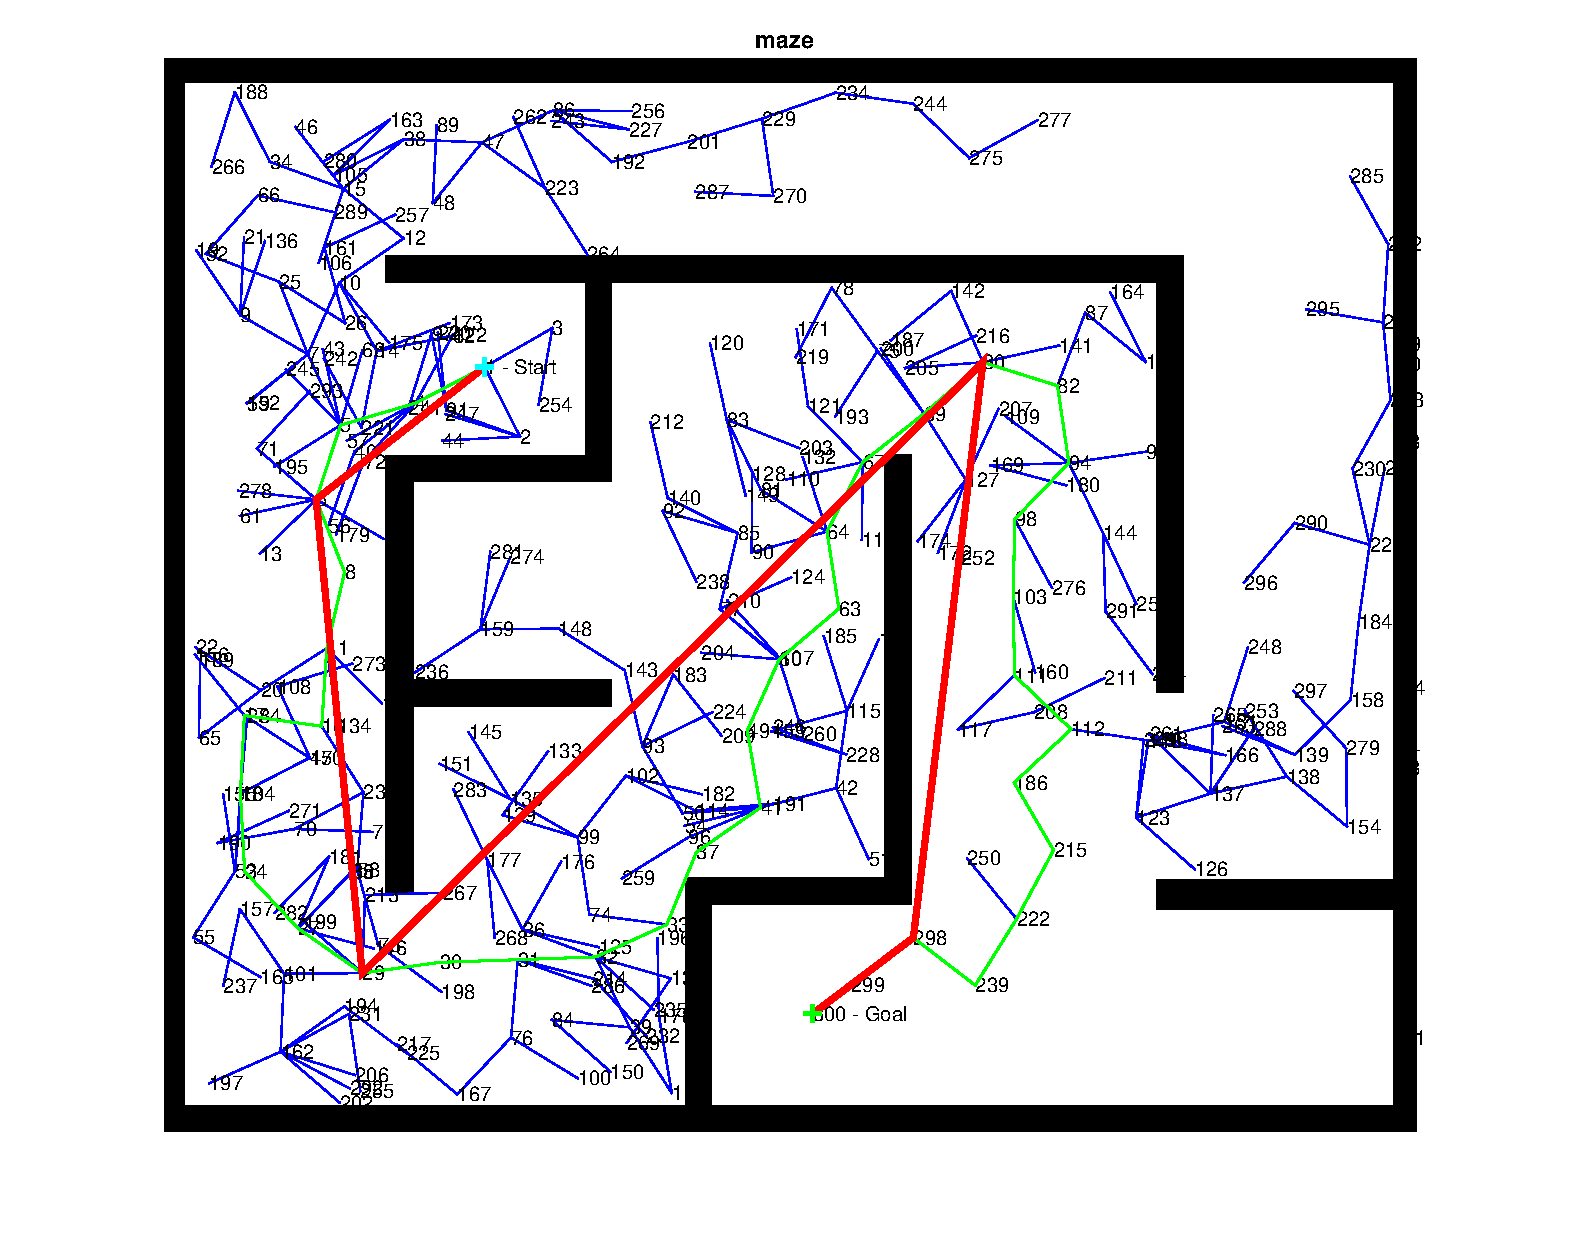
\includegraphics[width=0.45\linewidth]{figures/maze_50_03.eps}}\\		
		
	\subfigure[Map result with delta\_q=150]{\label{map150}
		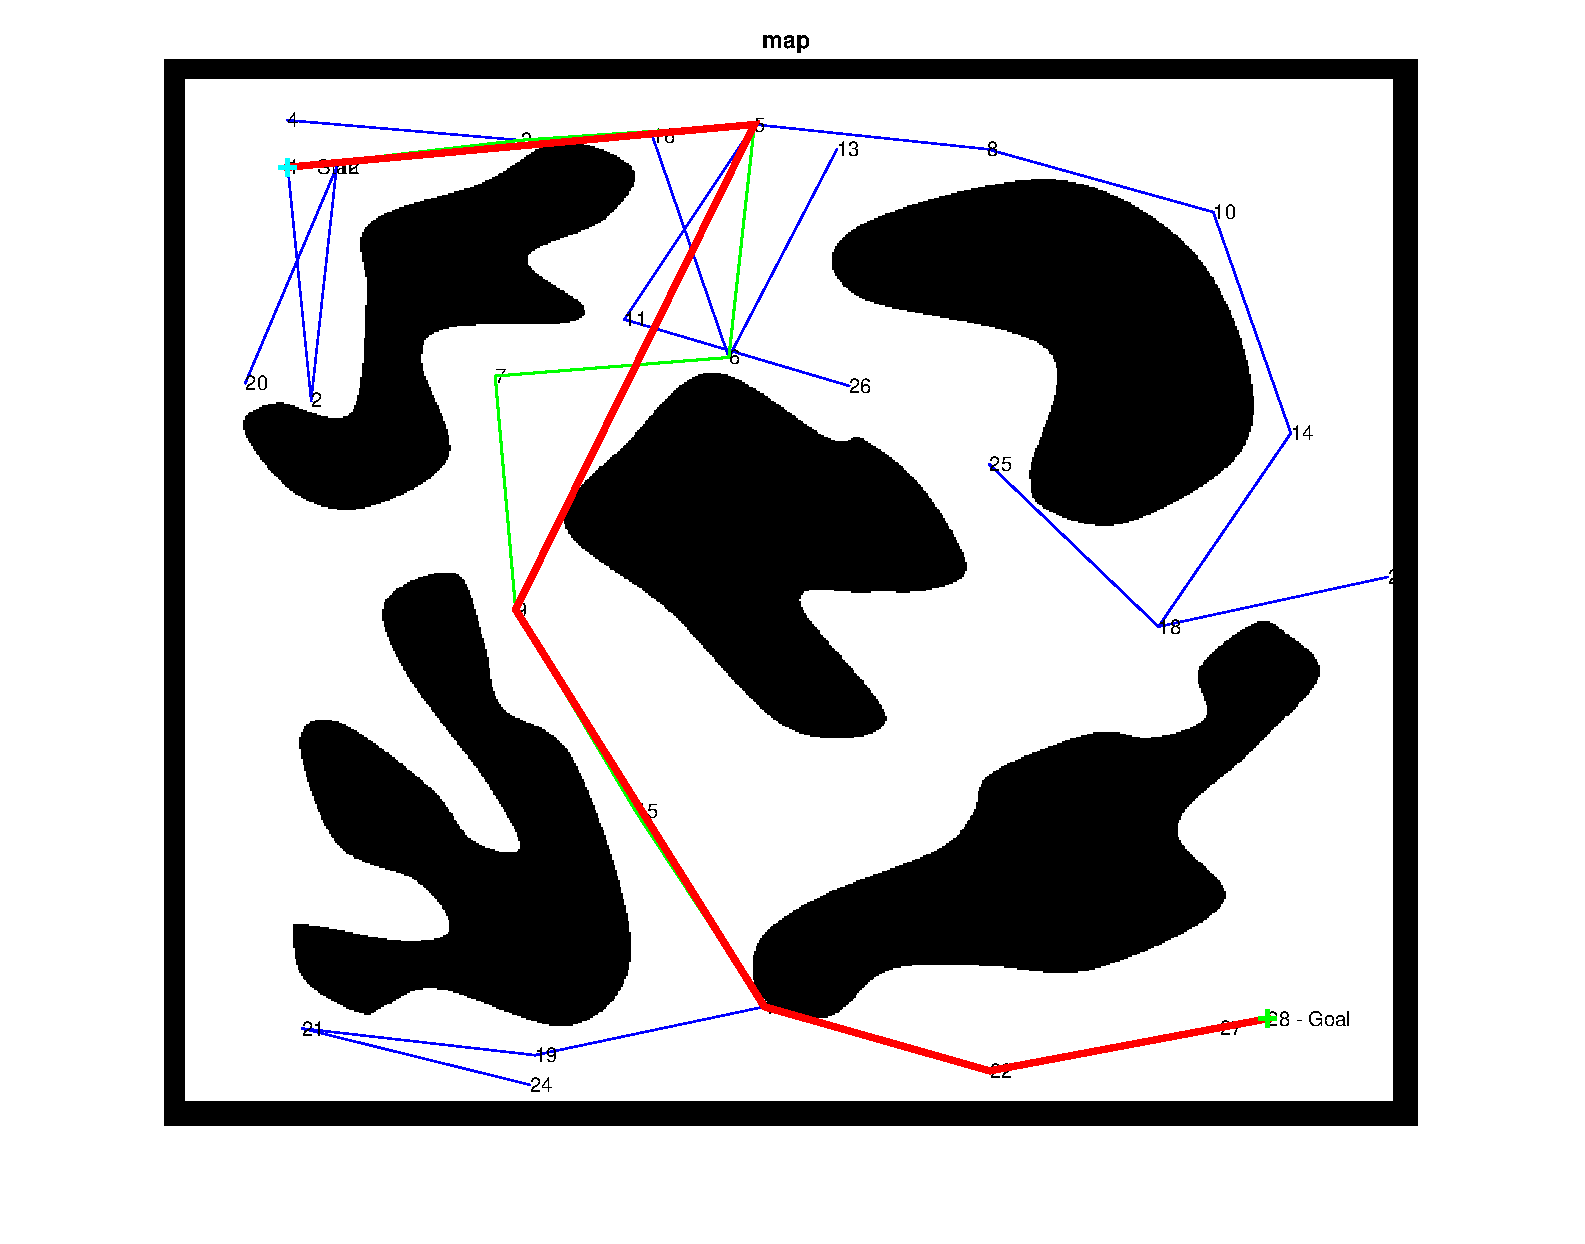
\includegraphics[width=0.45\linewidth]{figures/map_150_03.eps}}~
	\subfigure[Maze result with delta\_q=150]{\label{maze150}
		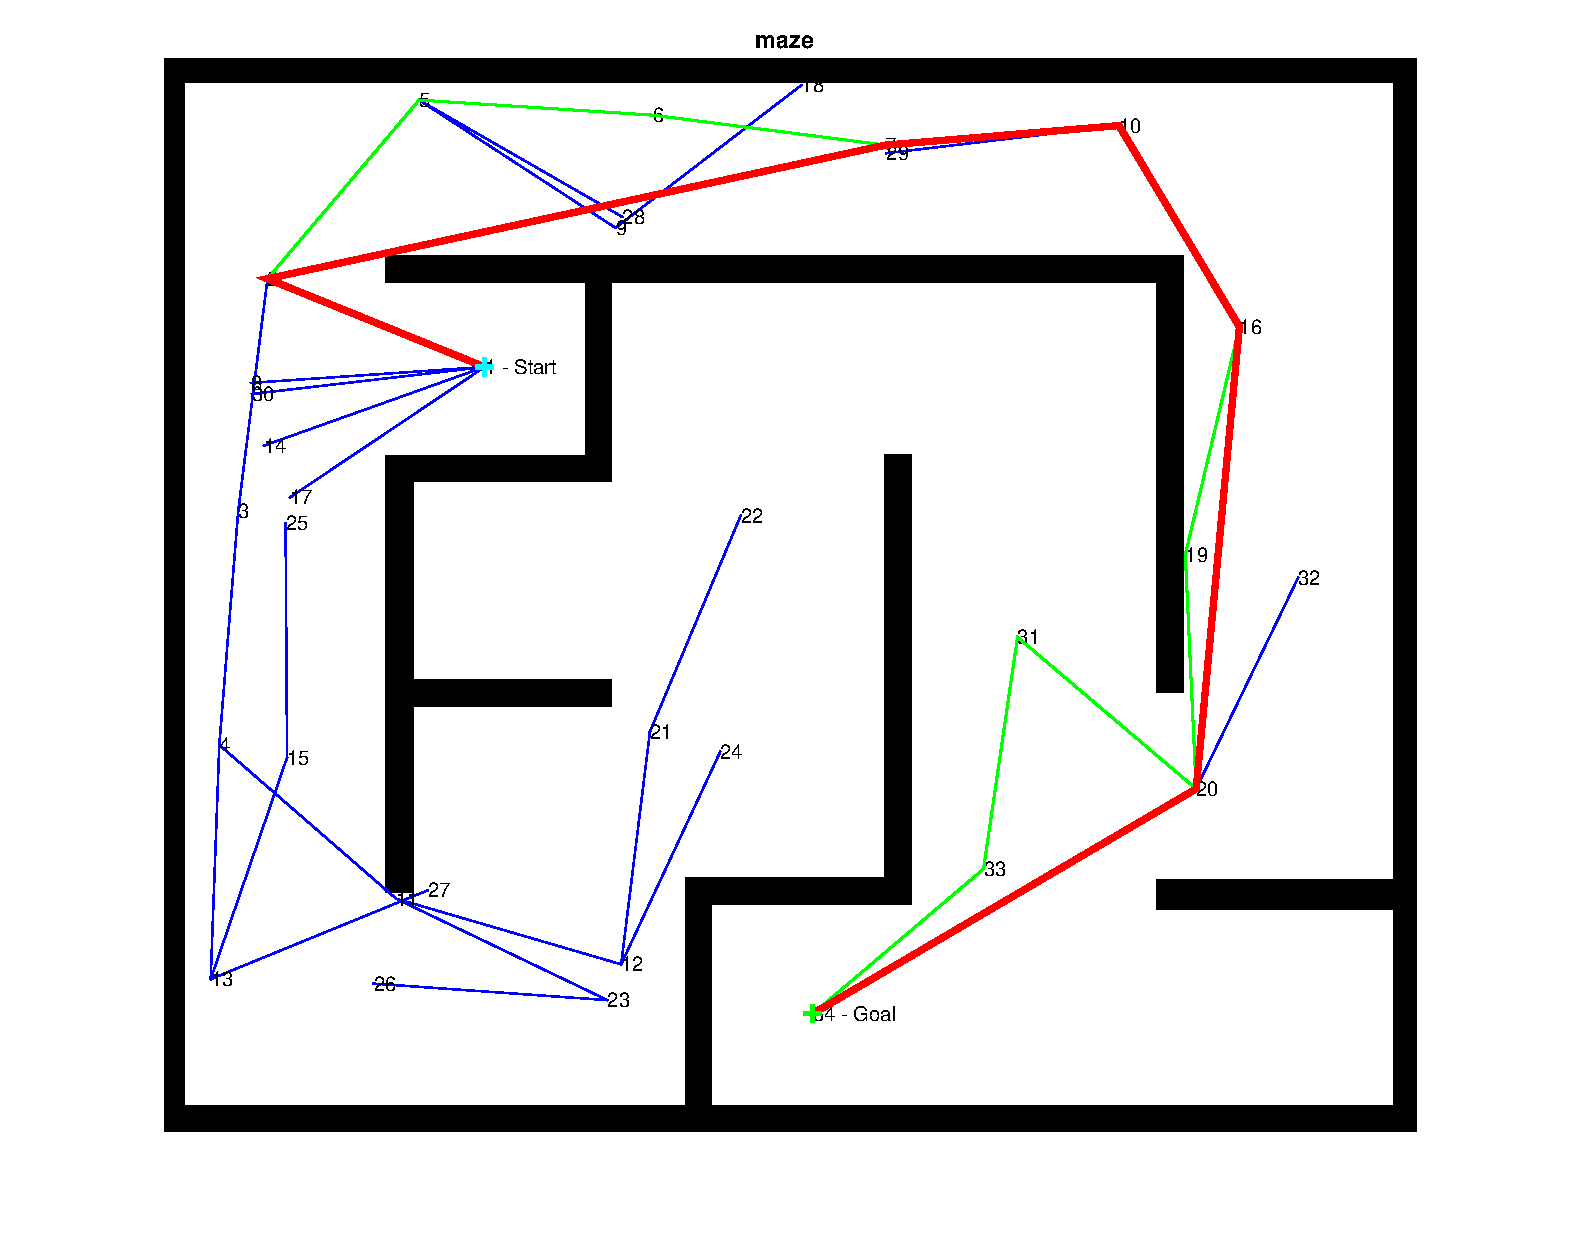
\includegraphics[width=0.45\linewidth]{figures/maze_150_03.eps}}\\		
		
	\subfigure[Map result with delta\_q=350]{\label{map350}
		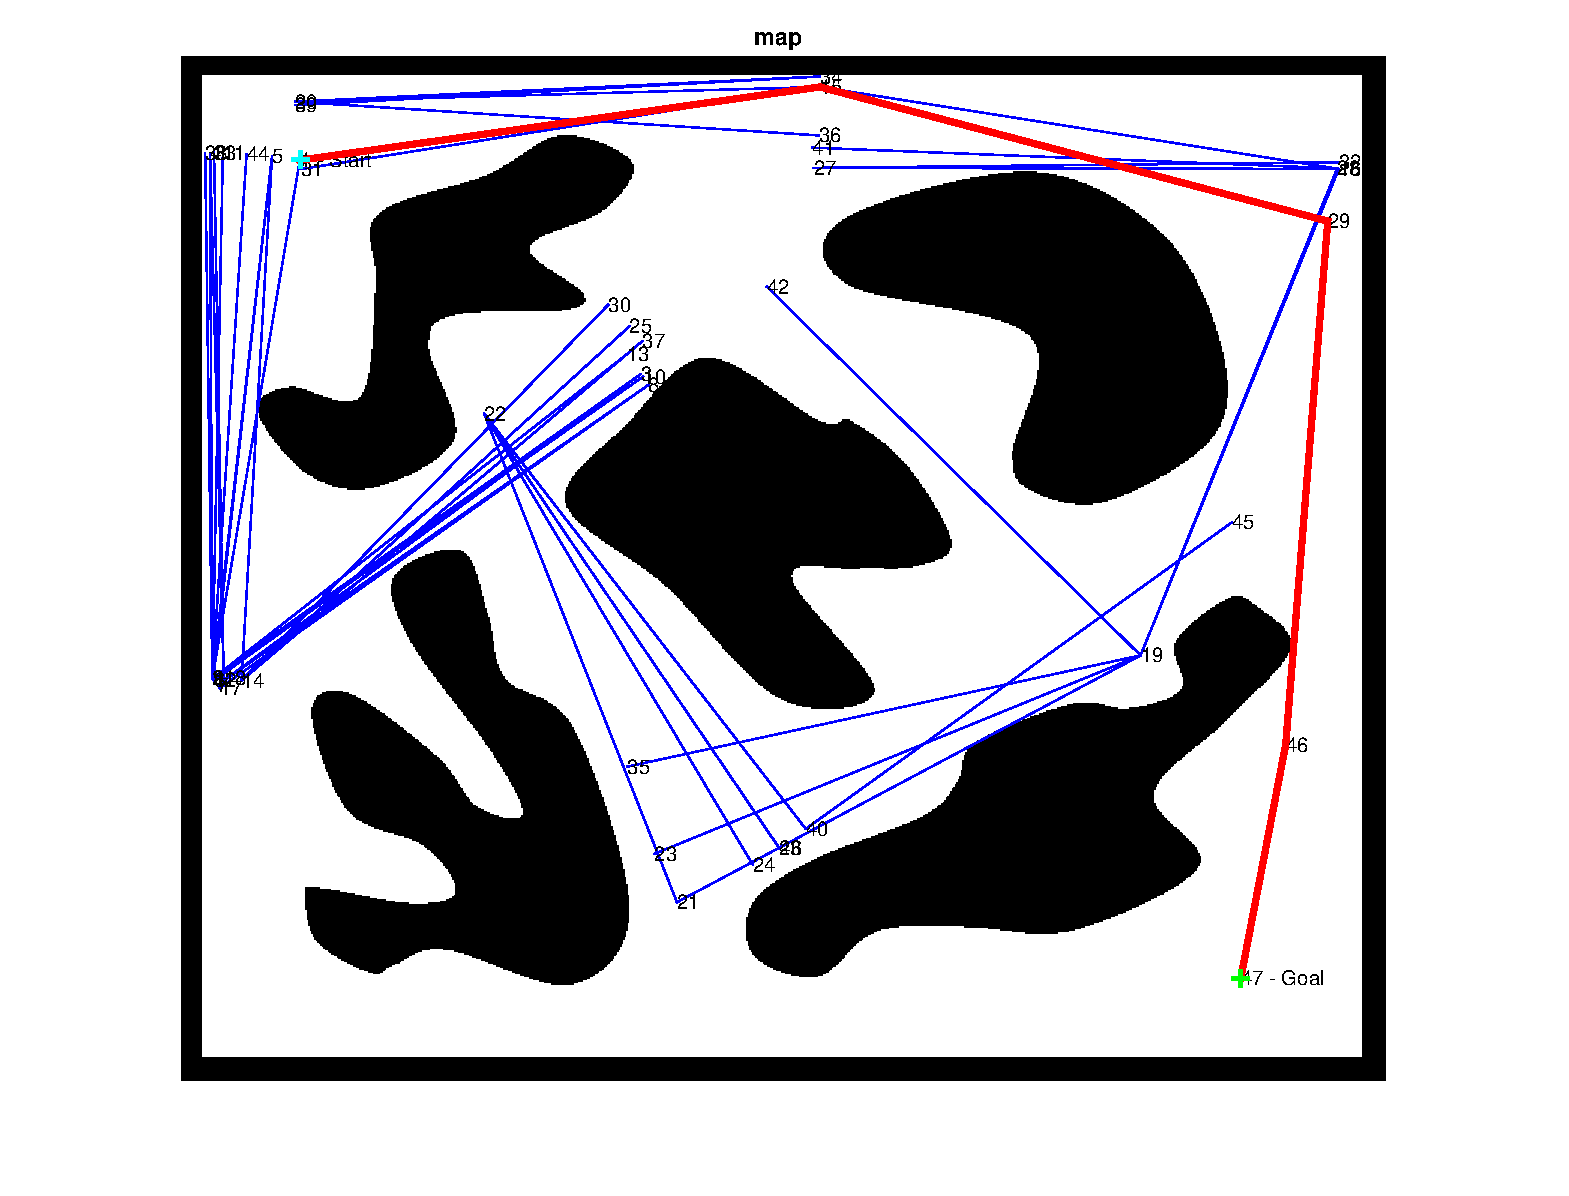
\includegraphics[width=0.45\linewidth]{figures/map_350_03.eps}}~
	\subfigure[Maze result with delta\_q=250]{\label{maze250}
		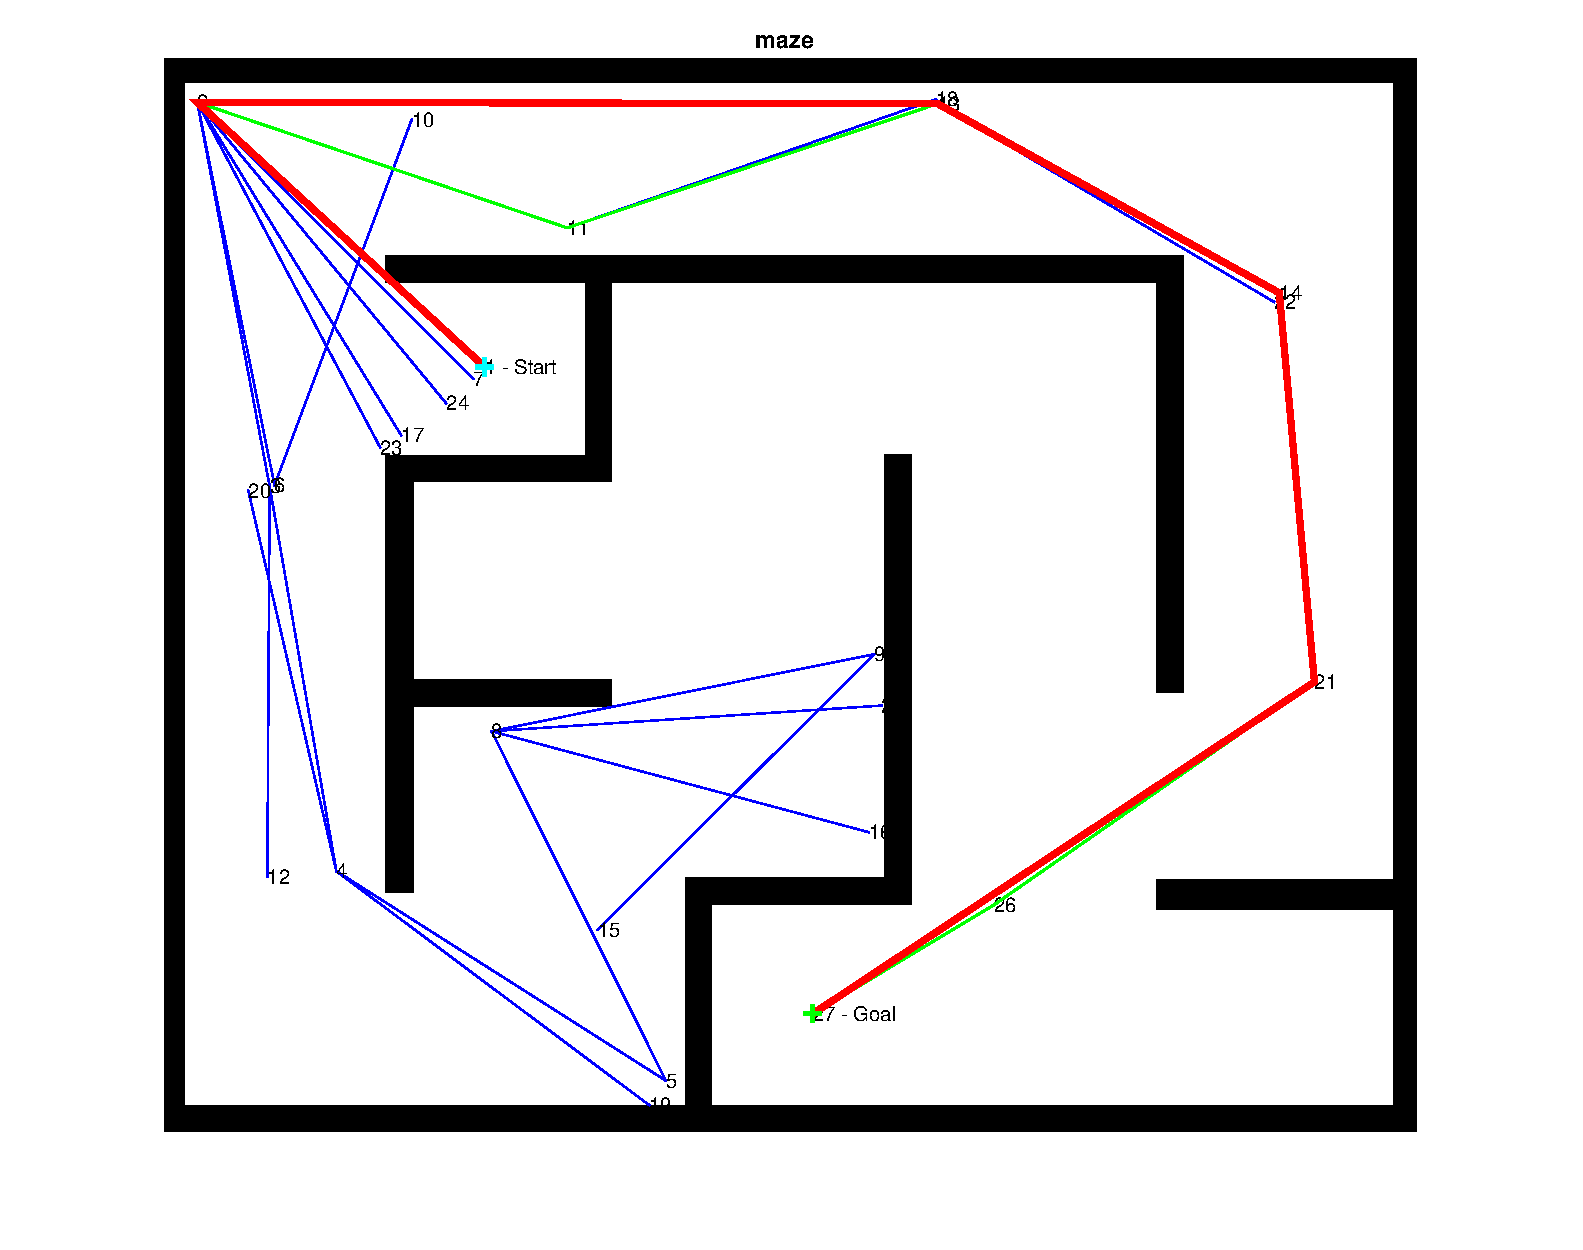
\includegraphics[width=0.45\linewidth]{figures/maze_250_03.eps}}\\
		
	\caption{RRT results for different delta\_q values}
	\label{fig:results}
\end{figure*}


Our \textit{rrt} and \textit{smooth} functions have been tested with two provided maps using different parameters for the \textit{rrt} function. Some results can be found in Fig. \ref{fig:results}, where the value of \textit{delta\_q} has been varied to observe the algorithm's behaviour. The value of \textit{p} in these examples was $0.3$. In the images, the blue graph represents the initial nodes and edges generated by the RRT algorithm, the green line is the initial path given by the \textit{rrt} function, and the red line is the final path obtained in the output of the \textit{smooth} function.

We observed that small values of \textit{delta\_q} generally leads to a more robust RRT run, but it takes more time to compute the graph (Figs. \ref{map50} and \ref{maze50}). Larger values of \textit{delta\_q} lead to a faster exploration of the map still with a very robust performance (Figs. \ref{map150} and \ref{maze150}), but if we use too large values for \textit{delta\_q} the algorithm no longer work in a fast manner since it is difficult to find new legal points (Figs. \ref{map350} and \ref{maze250}), and if we further increase the value of \textit{delta\_q} the RRT can no longer work in that map. We can therefore conclude that an appropriate value is a very important choice when using an RRT algorithm, and previous knowledge of the map is desirable. If nothing is known about the map in advance, perhaps a smaller value of \textit{delta\_q} should be chosen to ensure the robustness of the function, although it may not lead to the best speed that could be achieved with this algorithm.


%%%%%%%%%%%%%%%%%%%%%%%%%%%%%%%%%%%%%%%%%%%%%%%%%%%%%%%%%%%%%%%%%%%%%%%%%%%%%%%
\section{Conclusion}\label{conclusion}

We observed in this lab session how the RRT algorithm can be used to generate a path between two points in a given map. The results show that the RRT algorithm is very fast and can be used with a variety of maps, but its results are not guaranteed even if a path is theoretically possible. Very complicated paths may be very hard for stochastic methods such as RRT to find. We could also observe how the choice of the \textit{delta\_q} parameter influences the speed and robustness of the results, and that it should be wisely chosen before the application of the \textit{rrt} function.



\appendices
\begin{figure*}
\section{rrt.m}\label{aprrt}

\begin{verbatim}
function [vertices,edges,path]=rrt(map,q_start,q_goal,k,delta_q,p);
% RRT trajectory planning implementation
% Rodrigo Daudt
% 01/04/16

map = map'; % To solve problems between carthesian and matricial coordinates
s = size(map);

added_goal = false;

% Initialise arrays for outputs
vertices = zeros(k+1,2); vertices(1,:) = q_start;
edges = zeros(k,2);
path = zeros(1,k);
last_added_vertex = 1;

% Loop through RRT k times
for i = 1:k
    if rand() <= p
        q_rand = q_goal;
    else
        % New random point in considered range
        q_rand = max(rand(1,2).*s,[1,1]); % max used to avoid eventual 0 index
    end
%     vertices(i+1,:) = q_rand;

    % Find index of closest vertex to q_rand
    min_d = sum(s);
    index = 0;
    for vertex = 1:last_added_vertex
        dist_v = norm(q_rand - vertices(vertex,:));
        if dist_v < min_d
            min_d = dist_v;
            index = vertex;
        end
    end

    % Generate q_new at distance delta_q from closest vertex in direction
    % of q_rand and add to vertices list
    dxy = q_rand - vertices(index,:);
    q_new = vertices(index,:) + delta_q*dxy/norm(dxy);
    q_new(1) = min(max(q_new(1),1),s(1));
    q_new(2) = min(max(q_new(2),1),s(2));

    added = false;
    if is_visible(map,vertices(index,:),q_new)
        last_added_vertex = last_added_vertex + 1;
        vertices(last_added_vertex,:) = q_new;
        edges(last_added_vertex-1,:) = [last_added_vertex, index];
        added = true;
    end
\end{verbatim}

\end{figure*}


\begin{figure*}
\begin{verbatim}
    % Check if we reached the end
    % check distance from q_new to q_goal
    % if distance < delta_q create edge between q_new and q_goal
    if added == true
        if norm(q_new - q_goal) < delta_q
            if is_visible(map,q_new,q_goal)
                last_added_vertex = last_added_vertex + 1;
                vertices(last_added_vertex,:) = q_goal;
                edges(last_added_vertex-1,:) = [last_added_vertex,
                                                last_added_vertex-1];
                added_goal = true;
                break;
            end
        end
    end
end

% Clean vertices and edges arrays
vertices = vertices(find(vertices(:,1) ~= 0),:);
edges = edges(find(edges(:,1) ~= 0),:);
if numel(edges) == 0
    path = [];
    return;
end

%  Find trajectory
if added_goal == false
    path = [];
    return
end
path = last_added_vertex;
vertex = last_added_vertex;
while edges(vertex-1,2) ~= 1
    vertex = edges(vertex-1,2);
    path = [path vertex];
end
path = [path 1];

% If we want the trajectory from start to goal, uncomment:
path = fliplr(path);

end

function visible = is_visible(map,q,q_new)

x = ceil(linspace(q(1),q_new(1),21));
y = ceil(linspace(q(2),q_new(2),21));

visible = true;
for i = 2:21
    if map(x(i),y(i)) == 1
        visible = false;
        break;
    end
end
end
\end{verbatim}
\end{figure*}



\begin{figure*}
\section{smooth.m}\label{apsmooth}

\begin{verbatim}
function [path_smooth] = smooth(map_in,path,vertices,delta)
% Smoothes path given by RRT function

if numel(path) == 0
    path_smooth = [];
    return;
end

map = map_in';
path_smooth = path(1);
N = size(path,2);
reached_end = false;
last_added = 1;

while reached_end == false
    
    added = false;
    for i = N:-1:(last_added+2)
        if is_visible(map,vertices(path(last_added),:),vertices(path(i),:),delta)
            path_smooth = [path_smooth path(i)];
            last_added = i;
            added = true;
            break;
        end
    end
    
    if added == false
        path_smooth = [path_smooth path(last_added+1)];
        last_added = last_added + 1;
    end
    
    reached_end = last_added == N;
end
end

function visible = is_visible(map,q,q_new,delta)
d = norm(q - q_new);
num_steps = ceil(d/delta) + 2;

x = ceil(linspace(q(1),q_new(1),num_steps));
y = ceil(linspace(q(2),q_new(2),num_steps));

visible = true;
for i = 1:num_steps
    if map(x(i),y(i)) == 1
        visible = false;
        break;
    end
end
end
\end{verbatim}

\end{figure*}

%\bibliographystyle{IEEEtran}
%\bibliography{Template_Daudt}


\end{document}


